\section{Git operations}
In this section we explore some of the git operations. We try to do
so, in a different way, if comparing with other manuals. Normally the
manuals we see around just explain how to perform an operation. We
try to go further, so in this manual, we have divided our operations in
three parts. In the first part, we give a description about the
operation. In the second part, we give the pre-conditions, or in other
words, we explain in which conditions the operations can be performed.
Finally, in the last part of each operation, we show what is the
result of perform such operation.

\subsection{Add and Remove}
The operations add and remove are used to add and remove content from
index. As we have said before the index contains all the files and
contents to be added on the next commit.\\

\emph{Git} add does not refer directly to the file. Instead it is like
a map from file to content. If we have a file on the index and we
modify it on the working directory, for this modification to be visible
on the next commit, the file has to be added again to the index.\\

The remove operation removes a file from index, so it will not be
present if we perform a commit exactly after the remove. The removed
file besides of being removed from index, it will also be removed from the 
working directory (if it is still exists there).

\subsubsection{Pre requisites}

There are a few cases where Git prevents you from removing a file, and they are: 
\begin{itemize}
\item The file doesn't exist in the index.
\item Removing a file, when the file with it's current content 
doesn't exist in last commit.
\end{itemize}
The last restriction exists, to avoid the accidental deletion of files. Imagine the
case where you have a file 'x' with 10k lines of code. You add it to the index,
but, before committing you accidentally use 'git rm x'. Because Git erases from
the index and the working directory you would lose it permanently. \par

\subsubsection{Result}

\subsubsection{Examples}

In these figures, it is shown the process of adding a file to the index. Note
that both files showing represent the same file, but with different content at
a given time. So imagine that, after adding "File1", "File0" is added. "File1"
would be removed from the index (because there cannot be a file with different
contents in the index at any given state) and "File0" would be added. What was
just described was the representation of the update of the content of a file in the
index. \par
\begin{figure}[h] 
	\caption{Add operation}
	\centering
	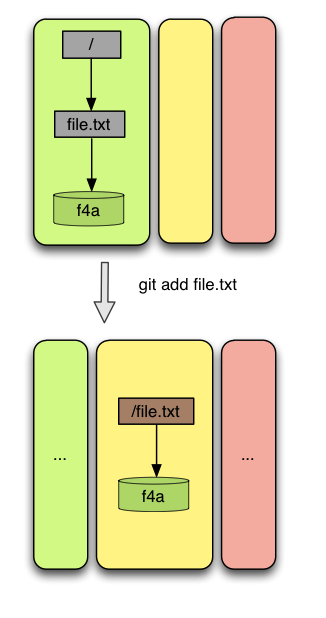
\includegraphics[scale=0.40]{images/add1.png}
\end{figure}

\begin{figure}[h] 
	\caption{Add operation (update)}
	\centering
	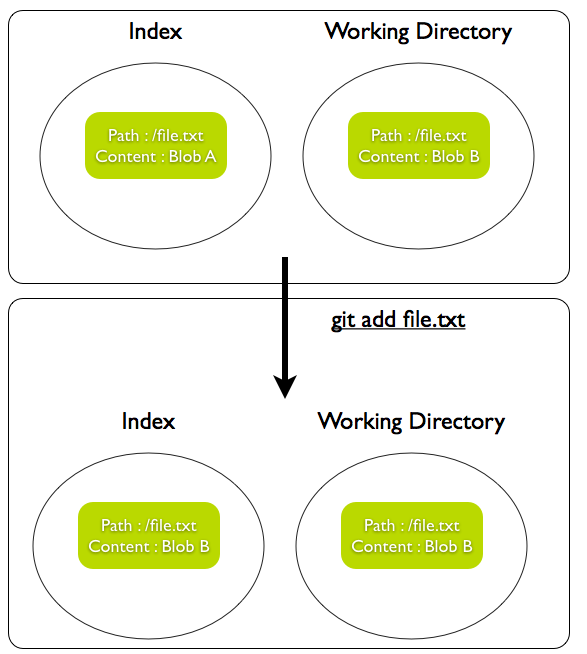
\includegraphics[scale=0.40]{images/add2.png}
\end{figure}

pagebreak
\pagebreak 

\begin{figure}[h] 
	\caption{Rm operation}
	\centering
	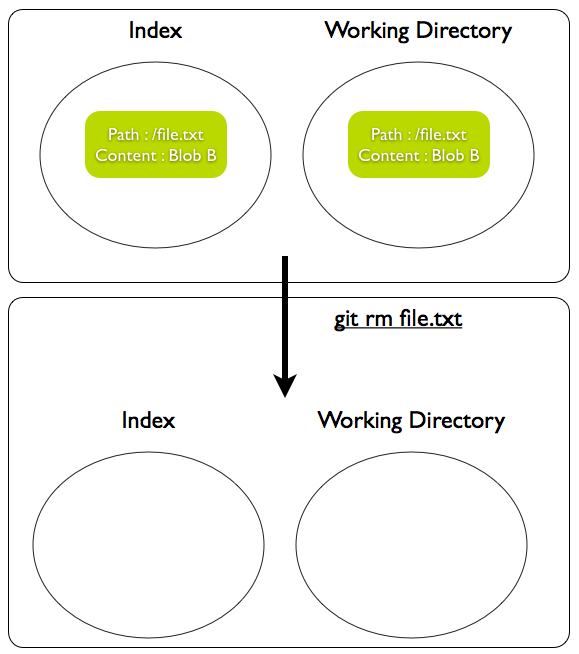
\includegraphics[scale=0.40]{images/rm1.png}
\end{figure}

pagebreak
\pagebreak 

\begin{figure}[h] 
	\caption{Rm operation (when the file doesn't exist in the Working
	Directory)}
	\centering
	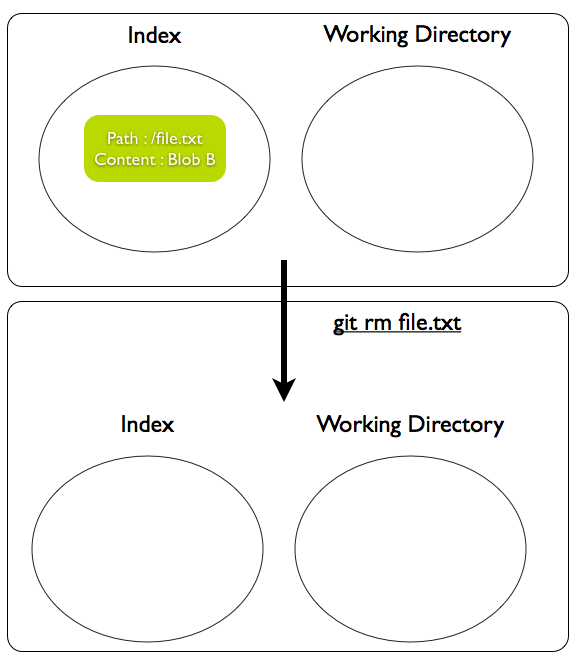
\includegraphics[scale=0.40]{images/rm2.png}
\end{figure}

pagebreak
\pagebreak 


\subsection{Commit}
The 'git commit' operation, stores the current content of the index in a new
commit. \par
When the first commit is created, a branch called "Master" will be created
and will be marked as the current branch. Also, the first commit of a repository
is called a RootCommit. \par

\subsubsection{Pre requisites}

The only restriction that Git has about this operation 
it's that your new commit must have something different from the previous
commit, or, if it's the first commit, then there must exist some content in
current index. \par


\subsubsection{Result}

\subsubsection{Examples}

%The figure \ref{fig:commit1} is a typical example of a RootCommit. There is a file with the path
%Name/Name, and a content Blob. It is currently on the index. The current branch
%is Master, and it is pointing to a commit, which represents the index at the current
%state. \par

pagebreak
\pagebreak

%\begin{figure}[h] 
%	\caption{A first commit}
%	\centering
%	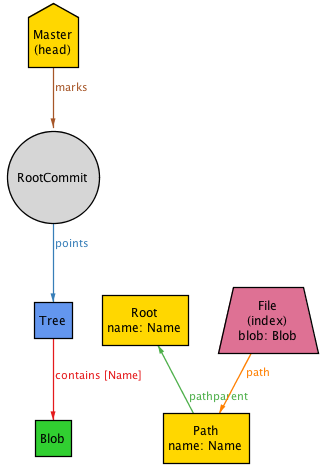
\includegraphics[scale=0.4]{images/commit1.png}
%	\label{fig:commit1}
%\end{figure}

pagebreak
\pagebreak



\begin{figure}[h] 
	\caption{A second commit}
	\centering
	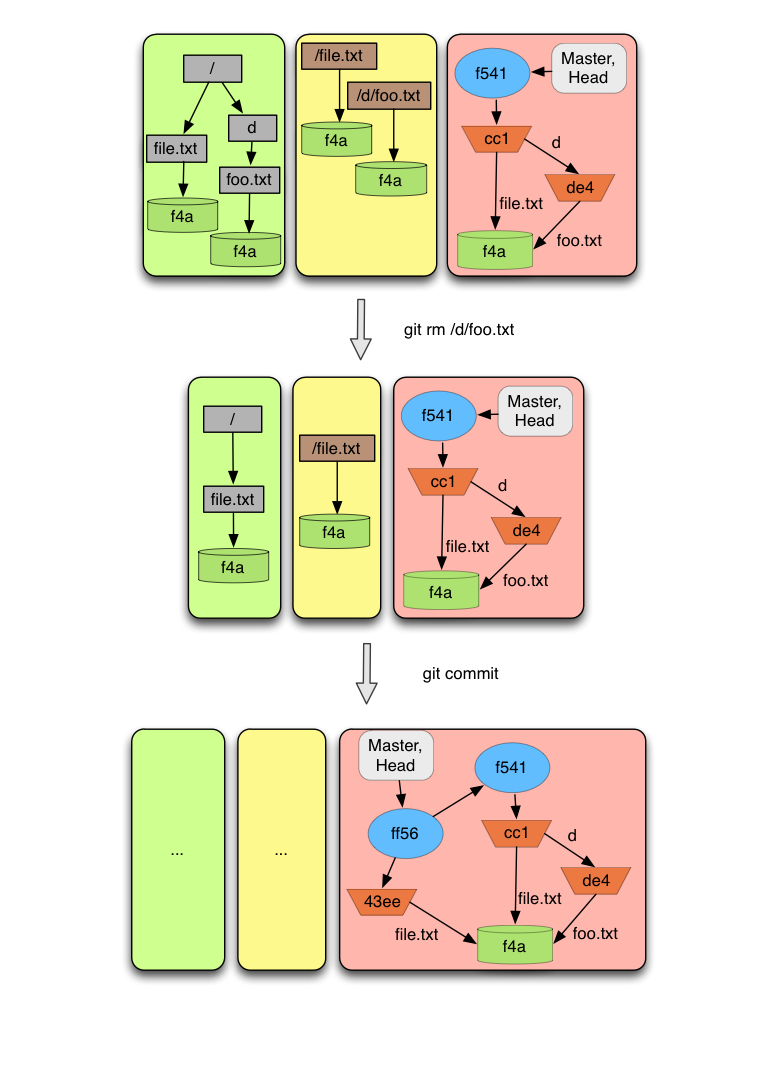
\includegraphics[scale=0.4]{images/commit2.png}
	\label{fig:commit2}
\end{figure}

The figure \ref{fig:commit2} represents the case of a normal commit, where the
newest commit comes after the RootCommit. The line of thought is the same as in
the last image. We can see that the difference between these two commits in the
figure, is that the only file was moved to a folder named "Name". \par
We can also see the efficiency of Git, about the sharing property of objects in
the commits, thus minimizing the space occupied in the repository. \par
\subsection{Branch}

\subsubsection{Pre requisites}

\subsubsection{Result}

\subsubsection{Examples}
Git branch operation has several forms, that to different things on git.
The ones which we care are the forms that create and delete branches. \par
When a new branch is created it will point to the current HEAD by default.
\par


The man git-branch says that when deleting a branch, it must be fully
merged in its upstream branch, or in HEAD if no upstream was set. \par


\subsection{Checkout}

\subsubsection{Pre requisites}

\subsubsection{Result}

\subsubsection{Examples}
From man git-checkout : "Switches branches by updating the index, 
working tree, and HEAD to reflect the specified branch or commit". \par

\subsection{Merge}


When you do a 'git merge <branch>', a merge will happen between the current
branch and the branch selected on the command. The result will be a new merge 
commit, or a partially merged index. \par

Git knows three types of merge : 
\begin{itemize}
\item A fast-forward merge, that will happen when 
the current commit from the other
branch, is more recent than the current commit from the current branch. \par
This type is not a true merge, in the sense that the only thing that
changes it's the pointer of the current branch
is moved to the newest commit.

\item A 2-way merge, that happens when the conditions for a fast-forward
don't exist, and there isn't a common ancestor for both commits.

\item A 3-way merge, happens when the conditions for a fast-forward
don't exist, but, there is a common ancestor for both commits. \par
The difference between these two last types, is that the last is much 
more automatic having much less conflicts than the previous type.
\end{itemize}
Knowing these 3 types of merge, it's important to know that Git tries to make
the merge process as automatic as possible. However conflicts do exist, and when
they happen it leaves to the user the process of resolving those conflicts. \par
When the Git/user, finishes the merging of files in the index, he
can commit the resulting merge, in a merge commit. \par
Note that while there are unmerged files in the index, a commit cannot be
made. \par 

\subsubsection{Pre requisites}

\begin{itemize}
\item A merge can't be made, if the current commit is more recent then the
other commit.
\item A merge can't be made, while there are unmerged files.
\item In the case of a fast-forward merge, the index can't have uncommitted
files that can be changed by the merge operation.
\item In the case of a 2-way or 3-way merge operation there can not be
uncommitted files. 
\end{itemize}

\subsubsection{Result}

\subsubsection{Examples}
\begin{figure} 
	\caption{A typical case of a fast-forward commit}
	\centering
	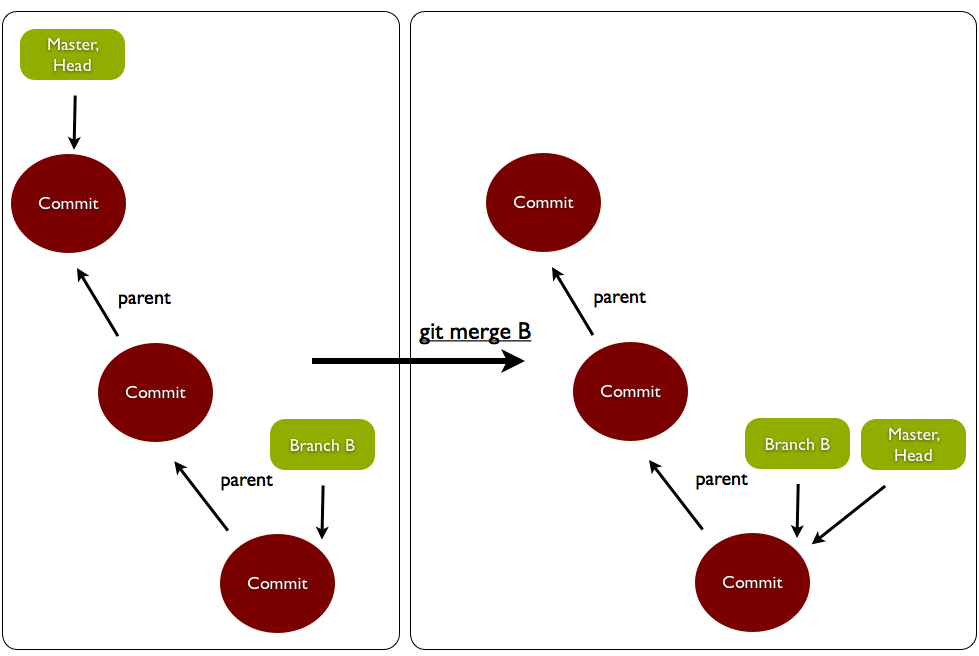
\includegraphics[scale=0.45]{images/fastforward.png}
	\label{fig:fastforward}
\end{figure}
\begin{figure} 
	\caption{Normal case of a 3-way merge}
	\centering
	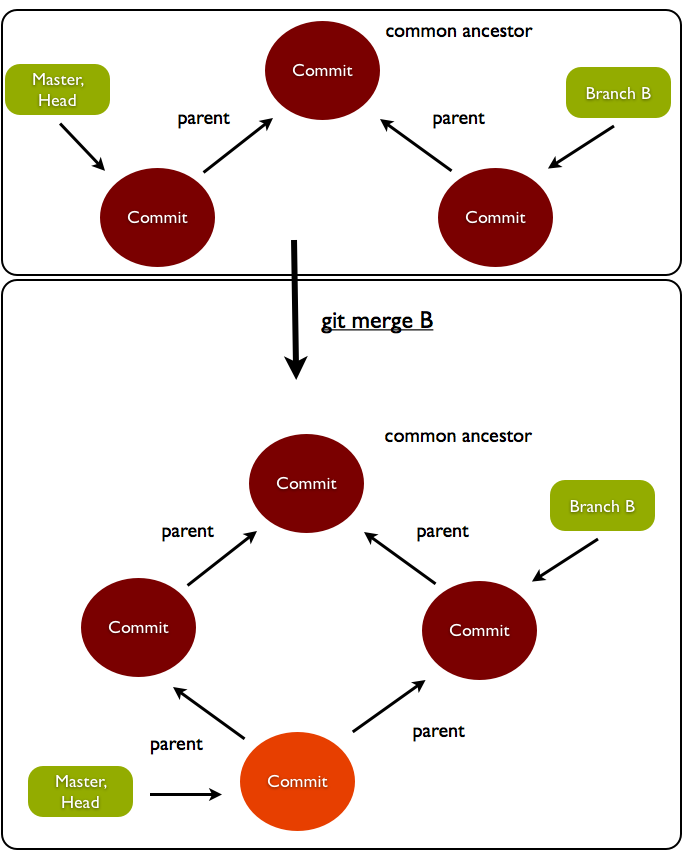
\includegraphics[scale=0.45]{images/normalmerge.png}
	\label{fig:merge}
\end{figure}
\begin{figure} 
	\caption{A case where, the merge operation can't be made}
	\centering
	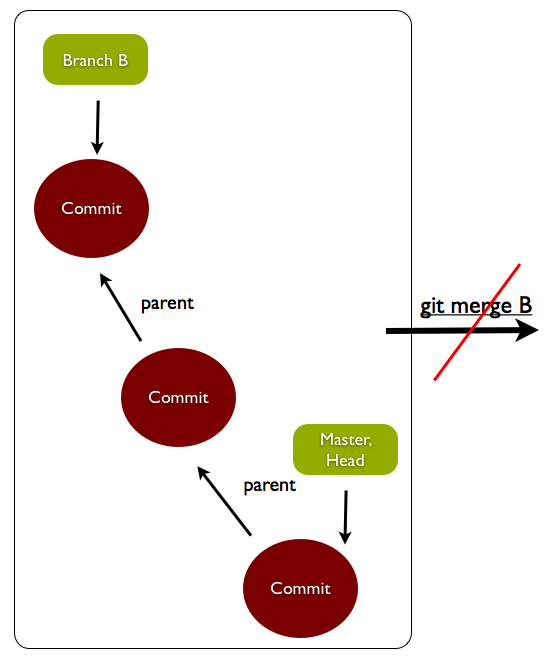
\includegraphics[scale=0.45]{images/nomerge.png}
	\label{fig:merge}
\end{figure}

\subsubsection{Git Pull and Git Push}

When working with remote repositories, these two operations will be vastly
used. They are in fact a sequence of operations, and are used to get content
from a remote repository and to place your content on the remote repository.
\par
If a 'git pull' is done, the branch from the remote repository will be fetched,
and the local branch and the remote branch will be merged. \par
If a 'git push' is done, the remote branch will be uploaded to the remote 
repository and will be merged there. \par
However, a 'git push' can only be done when the resulting merge will be a
fast-forward, simply because there is no one on the other side to resolve the 
merge conflicts. For the case of 'git pull' it's pre requisites are the same of
the merge operation. \par
